\documentclass[10pt,a4paper]{article}
\usepackage[margin=2cm]{geometry}
\usepackage{graphicx,booktabs,hyperref,xcolor,amsmath,subcaption,enumitem}
\hypersetup{colorlinks=true,linkcolor=blue!50!black,urlcolor=blue!50!black}
\graphicspath{{figures/}}
\setlist{nosep}

\title{\textbf{Team 4 --- Learning to Defend: Multi-Agent RL for Tello Counter-UAS}\\[2pt]
\large Action Space Hackathon (Microsoft NERD, Oct 23--25 2026) --- Technical Report}
\author{Team 4}
\date{October 25, 2026}

\begin{document}
\maketitle

\begin{abstract}
We trained reinforcement-learning policies in Isaac Lab for four Tello tasks: hover (T1), waypoint tracking (T2),
gate approach and landing (T4), and a 3-defender counter-UAS game (Defend). Every early RL run scored
near zero. We traced the cause to two pipeline bugs rather than to the reward design: a world-frame force
applied in the body frame, and \texttt{clip\_actions=True} in the skrl policy, which collapsed the learning rate.
With both fixed, the RL policies match or beat the scripted baselines:
T1 keeps the drone within 20\,cm of the target 91.6\% of the time (tail error 1.05\,cm),
T2 reaches 50.5\% within 20\,cm against 22.7\% for a PD controller, and T4 succeeds in 99.2\% of episodes against 89.1\% for the
organizers' policy. For Defend, a sparse-reward MAPPO curriculum passed gates S0--S2 and downs
8.13 attackers per episode at stage 2, against 8.07 for our best scripted strategy. The policy is a 53$\to$256$\to$128$\to$64 MLP.
It ships as a numpy-only file inside the organizers' \texttt{swarm\_ops} runner, behind a safety layer that stays on,
with the scripted strategy as a one-flag fallback.
\end{abstract}

\section{Problem and deliverable}
The organizers run 2--4 attacker Tellos and publish attacker and defender poses from an AprilTag-mapped room as a
UDP telemetry feed. Each team supplies \emph{one} Python policy that the organizers' host runs, sending \texttt{rc}
commands to three defender Tellos through USB WiFi dongles at about 13.5\,Hz.
The score is the number of attackers stopped (``downed'') before they reach a protected site (``breach'').
Table~\ref{tab:deliv} maps every deliverable to its location in the submission folder.

\begin{table}[h]\centering\small
\begin{tabular}{@{}ll@{}}\toprule
Deliverable & Location (\texttt{submission/}) \\\midrule
Defender package (install script, runner plug-ins, safety, tools) & \texttt{deploy/} (\texttt{install.sh}, \texttt{README.md}) \\
Primary Defend policy (RL, sparse S2) & \texttt{policies/defend\_rl\_sparse\_s2/policy.npz} \\
Alternate RL policies & \texttt{policies/defend\_rl\_sparse\_s3\_nogate}, \\ & \texttt{policies/aryan\_defend\_rl\_sparse\_s7\_c3} \\
Fallback (scripted assign-lead-safe) & \texttt{-{}-run defend\_lead:1,2,3} \\
T1 / T2 / T4 policies & \texttt{policies/\{hover\_t1, waypoint\_t2, approach\_r2\}} \\
Videos & \texttt{videos/\{sim3d, blender, isaac\}} \\
Plots and trajectories & \texttt{plots/}, \texttt{results/} \\\bottomrule
\end{tabular}
\caption{Submission map.}\label{tab:deliv}
\end{table}

\section{Simulation and training setup}
\textbf{Environments.} All tasks run in Isaac Lab with a Tello rigid-body model.
\texttt{AS-Defend-Live-v0} models what the real feed provides: attacker positions arrive delayed and noisy,
and velocities come from the same Kalman filter (\texttt{KalmanCV}) that runs on the host, so the policy sees in
training the same estimates it will see live. Stages 0--3 run a fast velocity-level dynamics model that matches the
Tello's \texttt{rc} interface.
\textbf{Observation} (53-d per defender): own state and heading, 4 attacker slots
$[\Delta p, \Delta v, \text{valid}]$ sorted in assignment order (so the input stays permutation-stable when the number of attackers changes),
and 2 teammate slots so the policy can learn spacing.
\textbf{Action}: body-frame velocity and yaw-rate (4-d), clamped to the \texttt{rc} range.
\textbf{Algorithm}: skrl MAPPO with a shared-architecture actor per defender, [256,128,64] ELU, running obs
normalisation, fixed LR $3\!\times\!10^{-4}$, $\gamma{=}0.99$, time-limit bootstrapping, 16{,}384 parallel envs.
\textbf{Reward}: sparse (take-down, wave cleared, breach, crash) with a curriculum ladder S0$\to$S6 that grows
attacker count, speed and evasiveness and shrinks the capture radius (S2 0.40\,m, S3 0.25\,m).
A stage \emph{gate} compares the policy to the best scripted baseline, assign-lead-safe, at the same stage over 256 episodes.
S1--S3 pass if the policy downs at least $0.95\times$ as many attackers, its breach rate is at most 2 points higher, and its crash rate is no higher.

\section{What made RL work}
Six initial Defend runs (MAPPO/IPPO, default and hard) and the first T1/T2 runs all failed in the same way. Returns fell
\emph{below} the zero-action policy, the KL-adaptive learning rate collapsed from $10^{-3}$ to roughly $0$ in a few
iterations, and the drones climbed away. We found two bugs:
\begin{enumerate}
\item \textbf{Frame bug.} A world-frame force was passed to \texttt{set\_external\_force\_and\_torque}, which expects
the body frame. After the fix, a random policy scores about the same as the zero-action policy (+6.7 vs +6.0) instead of $-90$.
\item \textbf{\texttt{clip\_actions=True}} on the skrl Gaussian policy produced a vanishing gradient through the clip,
which in turn drove the learning-rate collapse (and NaN weights with a fixed LR). Setting it to \texttt{False} with a fixed LR fixed T1 at once.
\end{enumerate}
We also removed two reward exploits in the Defend environment: a suicide dive that scored kills by colliding, and a
$\gamma{=}0.99$ potential-shaping leak that paid +54 per episode for hovering. After that, no probe policy beat doing nothing.
Figure~\ref{fig:fixes} shows the effect of the fixes.

\begin{figure}[h]\centering
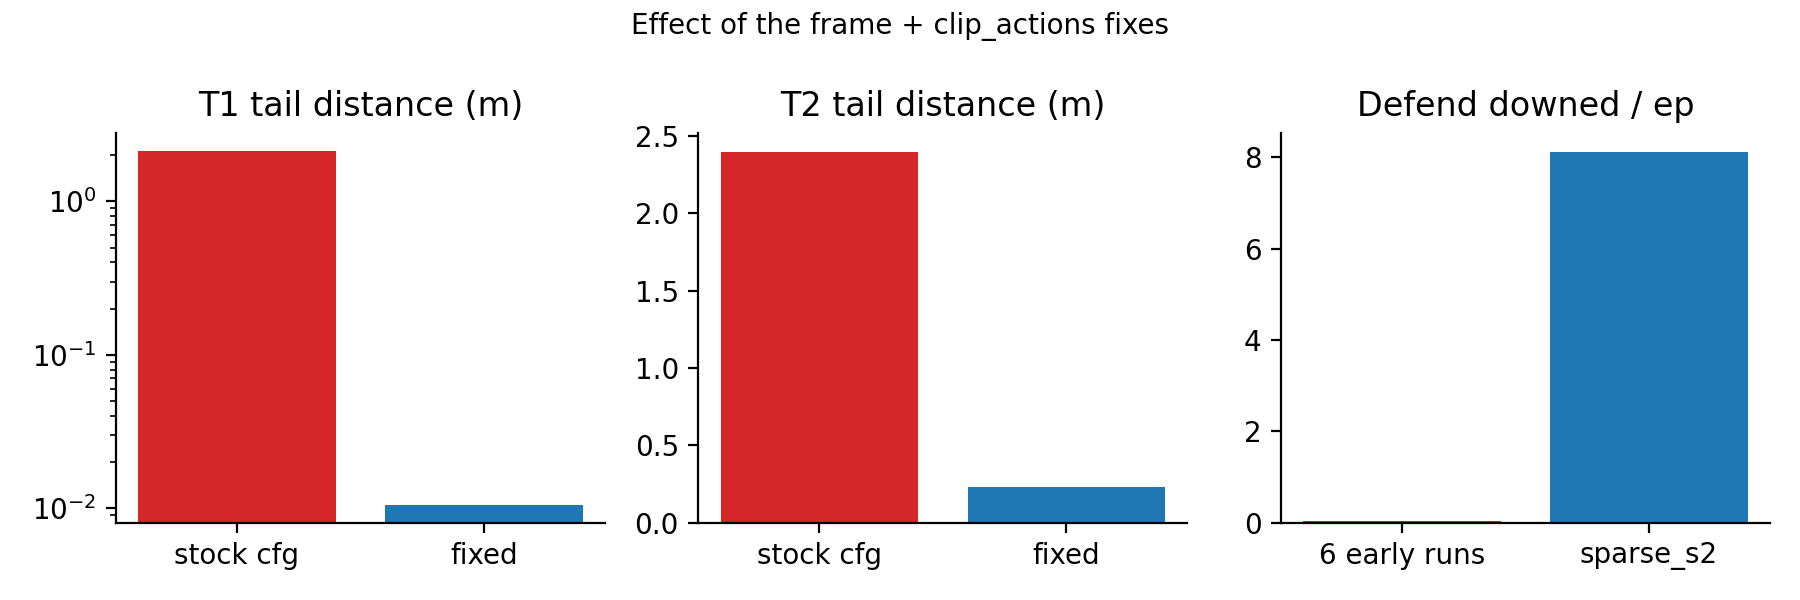
\includegraphics[width=.92\linewidth]{fig_fixes.png}
\caption{Before and after the pipeline fixes (same tasks, same evaluation).}\label{fig:fixes}
\end{figure}

\section{Results}
\subsection{Basic tasks (T1, T2, T4)}
\begin{table}[h]\centering\small
\setlength{\tabcolsep}{4pt}\footnotesize\begin{tabular}{@{}lllll@{}}\toprule
Task & Policy & Metric & Ours & Baseline \\\midrule
T1 Hover & skrl PPO, 400 it & \% time $<$20\,cm / tail dist & \textbf{91.6\% / 0.0105 m} & PD 96\% / 0.0001 m; zero 13\% \\
T2 Waypoint & skrl PPO, 3000 it (W1) & \% time $<$20\,cm / tail dist & \textbf{50.5\% / 0.218 m} & PD 22.7\% / 0.305 m \\
T4 Approach & SB3 PPO, r2 & success / collision & \textbf{0.992 / 0.004} & shipped it5 0.891 / 0.008 \\\bottomrule
\end{tabular}
\caption{Basic tasks, 256--512 episodes, seed 7. Zero deaths in every RL run.}\label{tab:basic}
\end{table}
On T1 the RL policy comes close to an ideal PD hover. On T2 it beats PD by $2.2\times$ on time within 20\,cm.
Training $3.75\times$ longer gained only 6\%, and adding a goal-velocity observation \emph{hurt}
(34.5\%), so we closed T2 at W1. T4 round 2 continued round 1 at a lower LR and cut collisions by $5\times$.

\begin{figure}[h]\centering
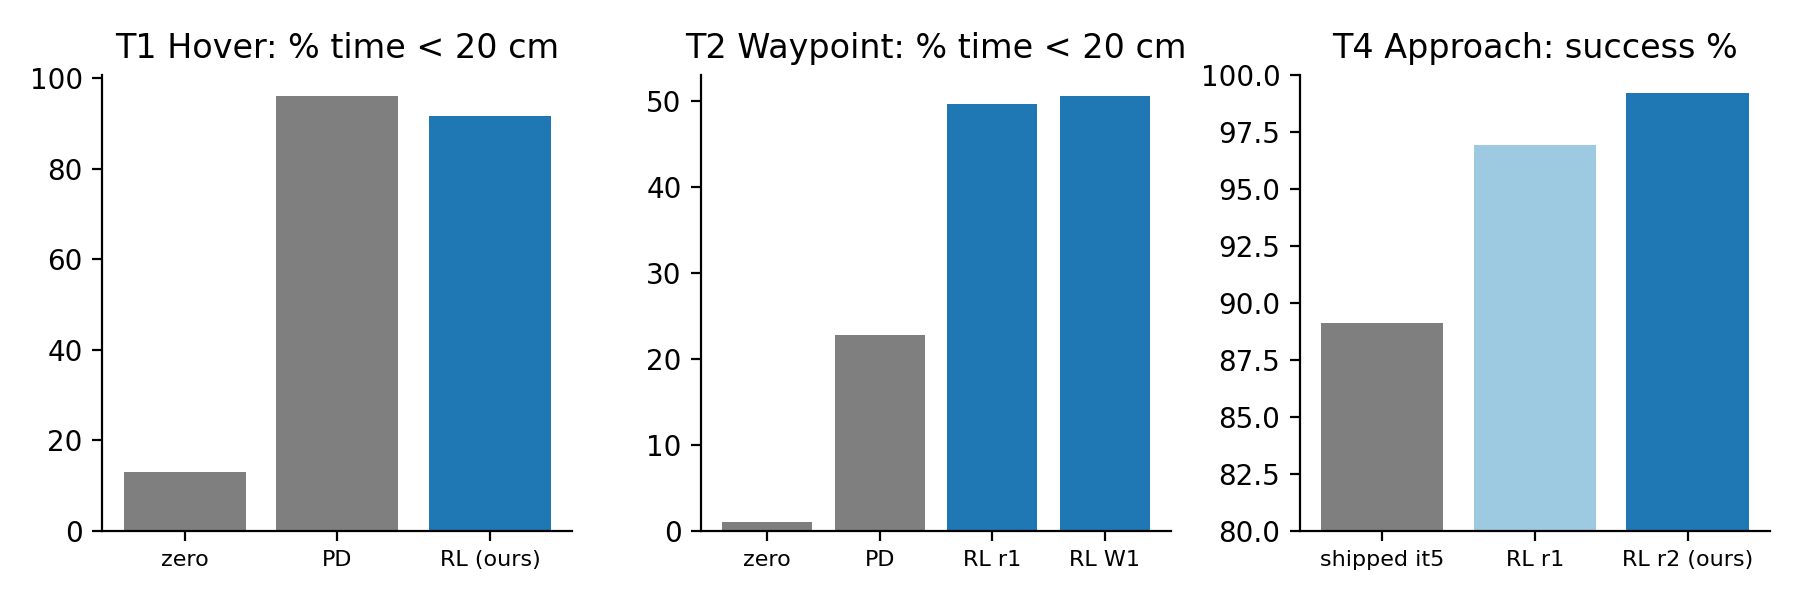
\includegraphics[width=.92\linewidth]{fig_basic_tasks.png}
\caption{RL policies against scripted and shipped baselines.}\label{fig:basic}
\end{figure}

\subsection{Defend (3 defenders vs N attackers)}
Figure~\ref{fig:gates} shows the curriculum gates. The dense-reward line passed S0 (7.36 vs 6.91) but failed S1 on
crashes: with $r_\text{crash}{=}-10$ about equal to one capture, a collision that wins a kill breaks even.
The sparse line passed S0--S2. For S2, earlier tries had collapsed the action std to 0.03--0.06, so we
re-inflated it to 0.4 on warm start, and the policy then passed with \textbf{8.125 downed/ep} against 8.066. At S3 the policy downs \emph{more}
attackers than the scripted baseline (8.31 and 8.58 vs 7.98) but crashes 0.15 times per episode against a 0.05 gate, so it fails twice.
An adaptive curriculum addresses this. On each gate failure it interpolates the stage difficulty
$\alpha\in[0,1]$ between S$_{k-1}$ and S$_k$ and strengthens the crash penalty, then steps $\alpha$ back up.
It was still running on two seeds when we submitted.

\begin{figure}[h]\centering
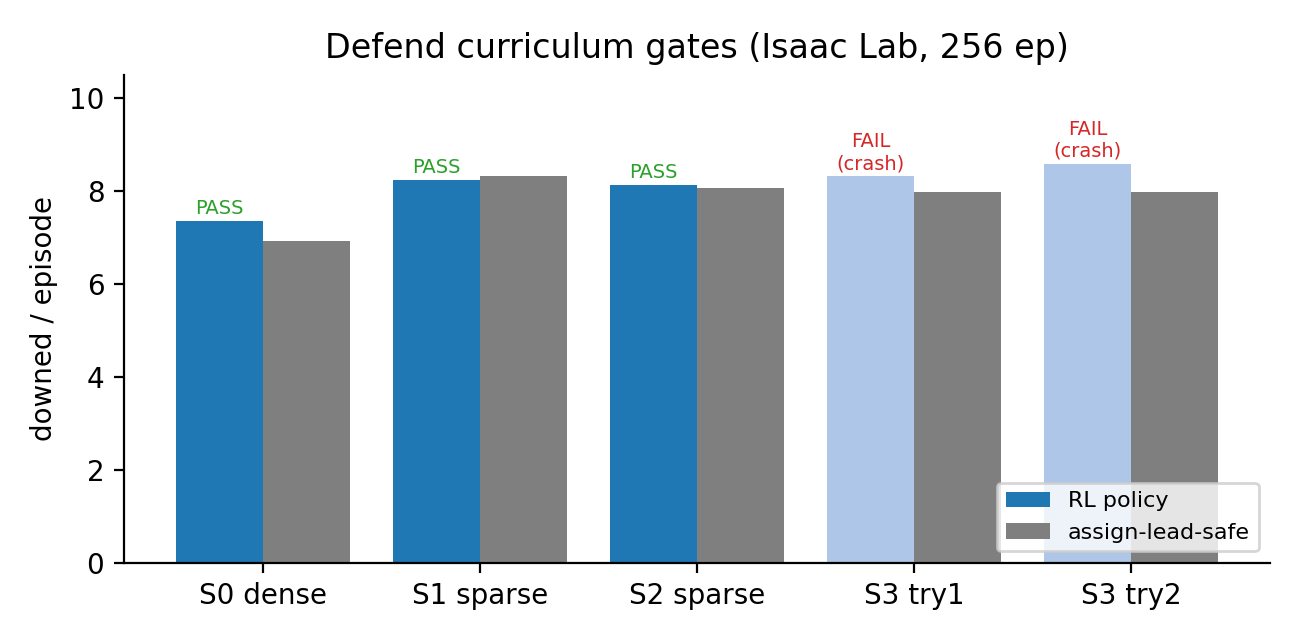
\includegraphics[width=.7\linewidth]{fig_defend_gates.png}
\caption{Isaac Lab gates, policy vs assign-lead-safe at the same stage (256 episodes). S1 passes under the relaxed
$0.95\times$ rule. S3 fails on the crash rate, not on take-downs.}\label{fig:gates}
\end{figure}

\textbf{Sim-to-deploy parity.} The deploy path (\texttt{defend\_live.py} / \texttt{swarm\_ops}) is pure numpy. Exported
weights match torch to $7\times10^{-15}$ (fp64). We re-ran the full deploy pipeline, including the delayed and noisy feed, Kalman
filter, safety layer and per-axis speed clamp, in closed loop against the same stage generator (Fig.~\ref{fig:stages}).
At S2 it gives 8.20 downed/ep against 8.125 in Isaac. The earlier 17--20\% gap came from a safety cap on the norm of the xyz velocity
(1.0), whereas the env clamps each axis ($\sqrt3$). Fixing that closed the gap. The policy beats the scripted baseline at S0--S2 in this
harness but loses at S3 (4.77 vs 7.92, 48\% breach). For that reason we keep assign-lead-safe as a one-flag fallback and check it in the venue dry-run.
Policy inference has a p99 latency of 1.9\,ms per tick.

\begin{figure}[h]\centering
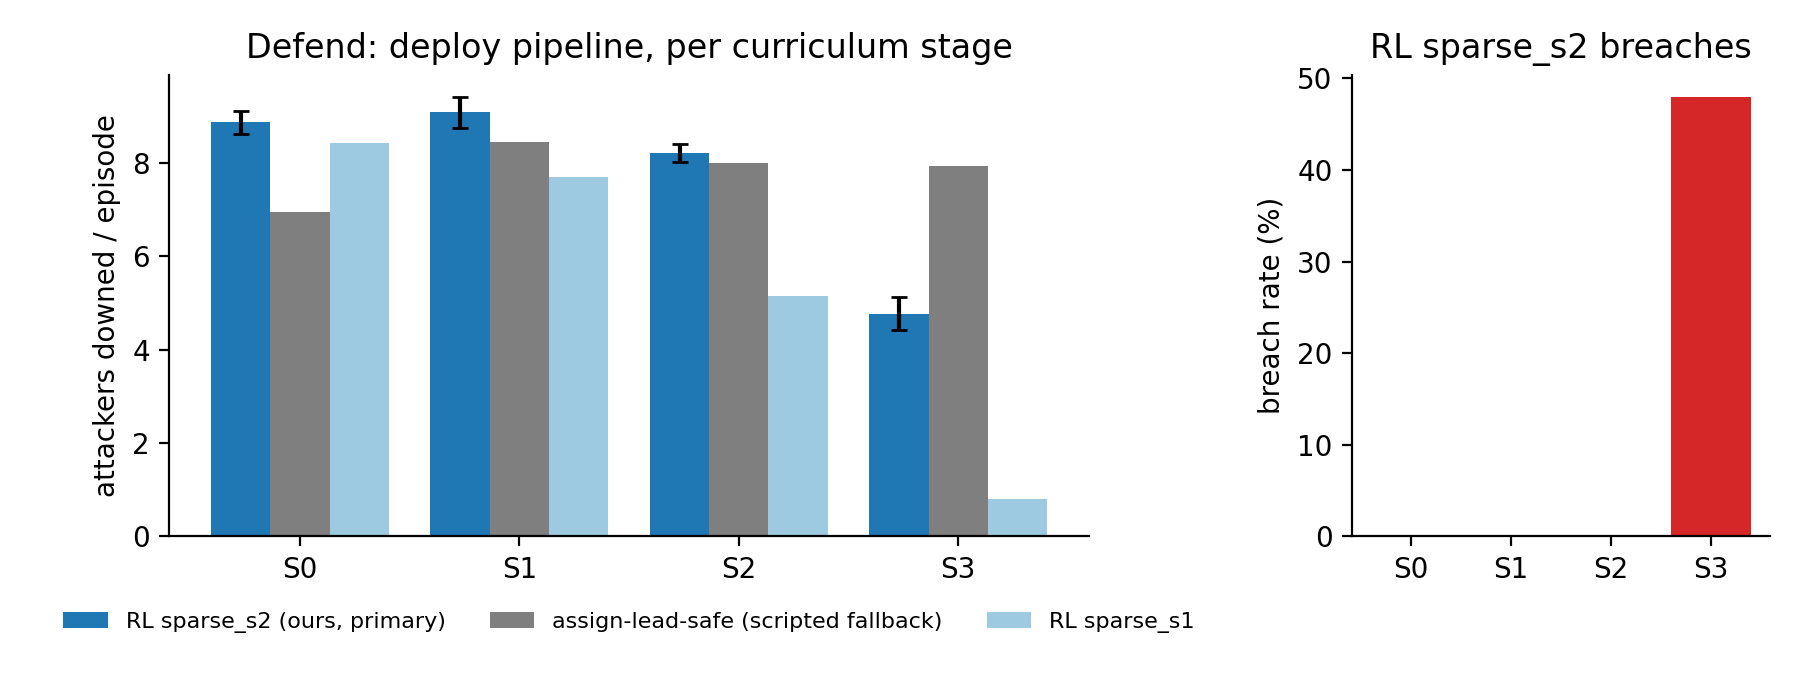
\includegraphics[width=.95\linewidth]{fig_defend_stages.png}
\caption{Closed-loop deploy pipeline (\texttt{defend\_live -{}-dry-run -{}-feed stage:K}, 64 episodes).}\label{fig:stages}
\end{figure}

\begin{figure}[h]\centering
\begin{subfigure}{.24\linewidth}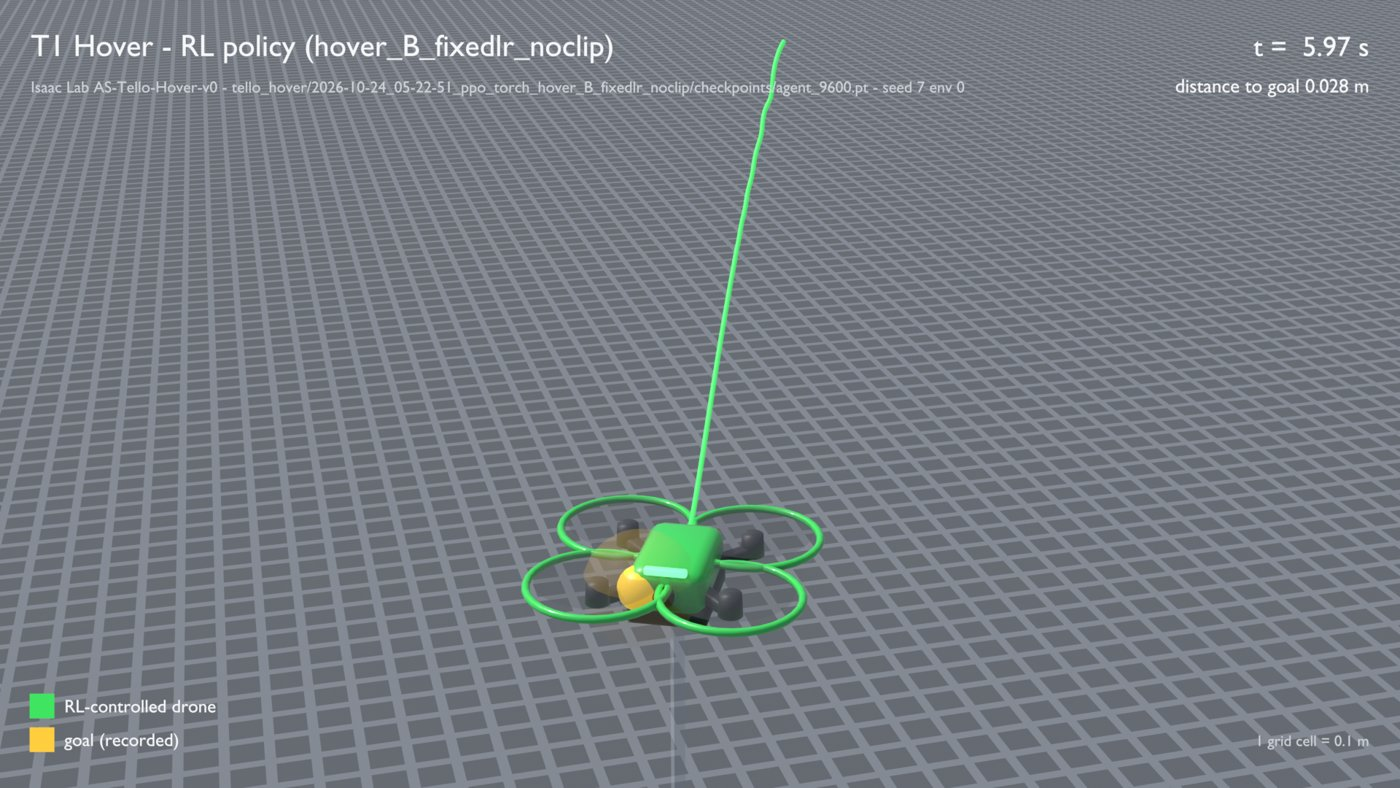
\includegraphics[width=\linewidth]{blender_t1.jpg}\caption{T1 hover}\end{subfigure}
\begin{subfigure}{.24\linewidth}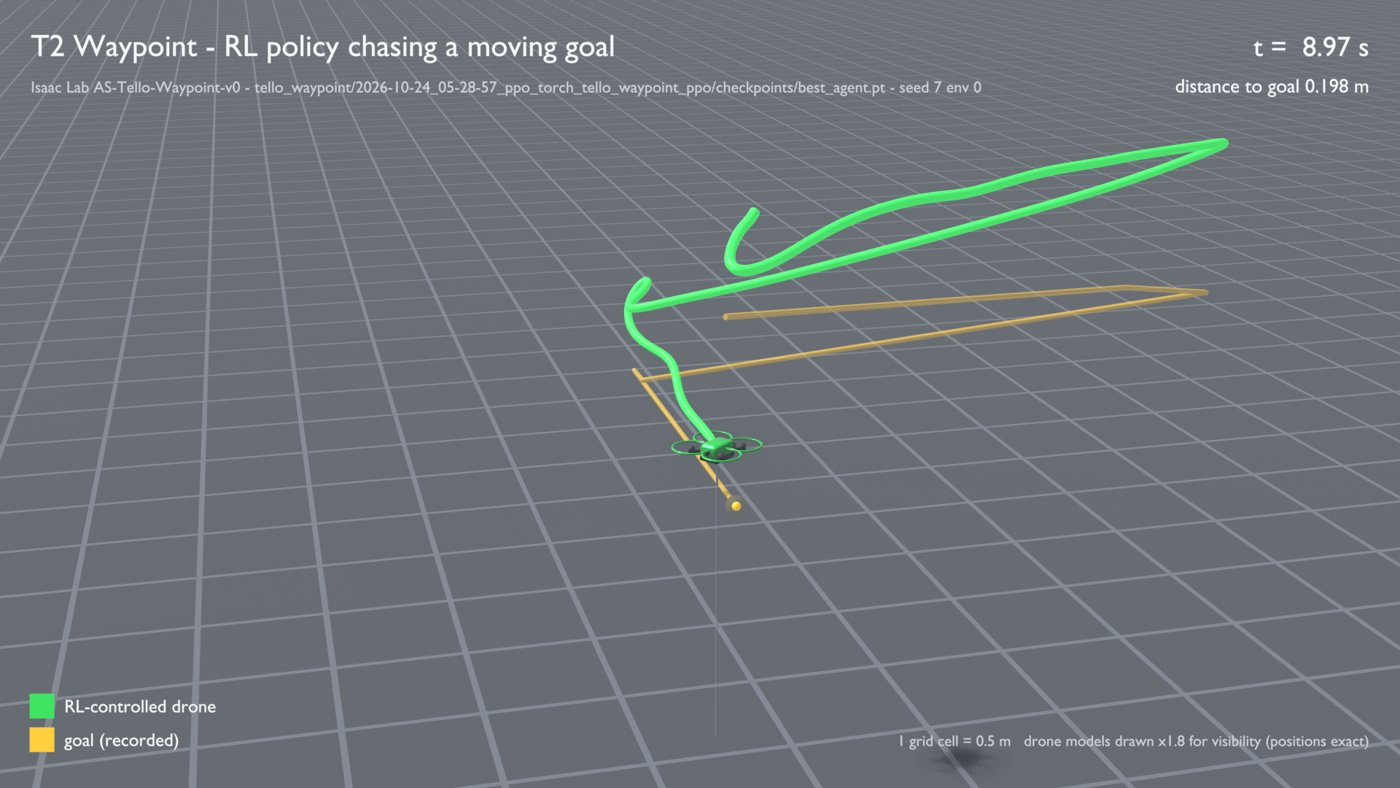
\includegraphics[width=\linewidth]{blender_t2.jpg}\caption{T2 waypoint}\end{subfigure}
\begin{subfigure}{.24\linewidth}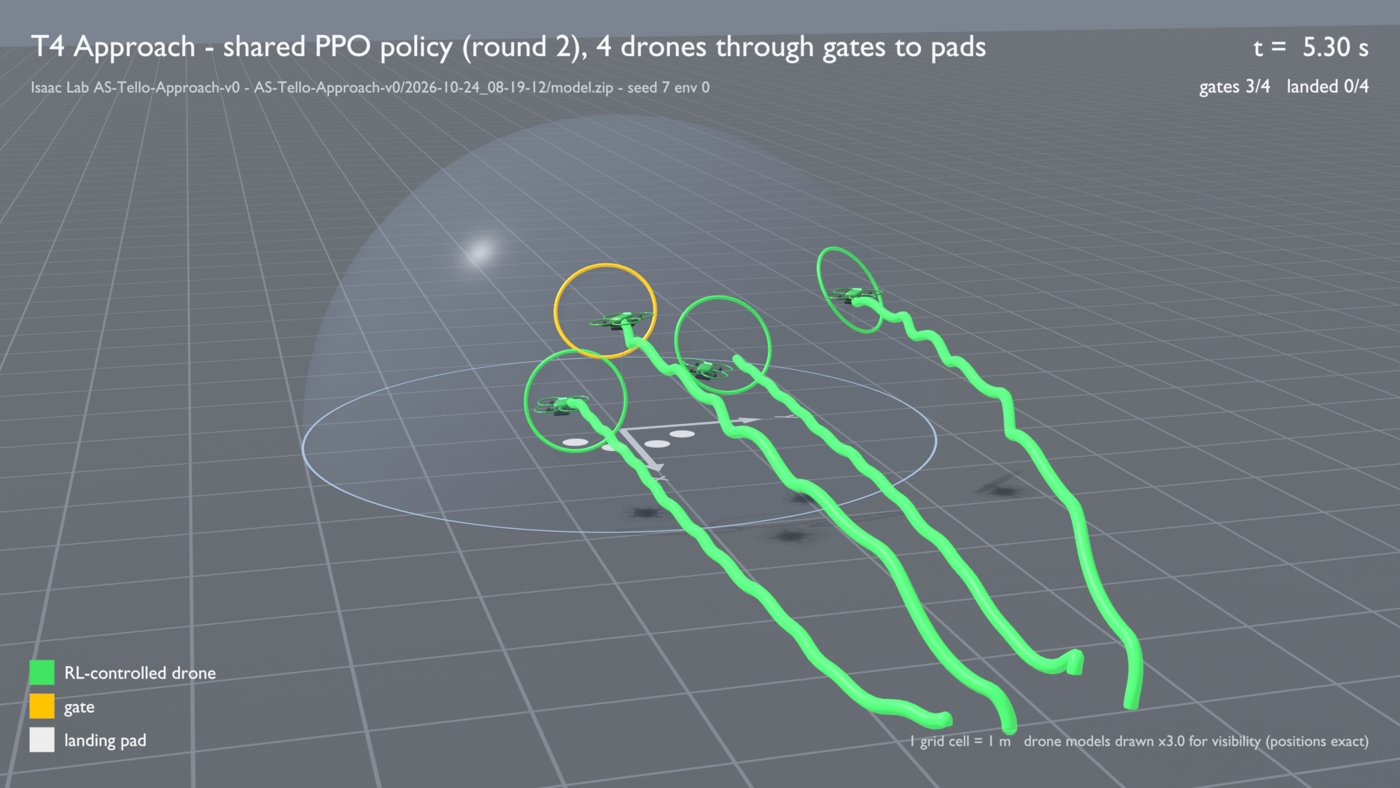
\includegraphics[width=\linewidth]{blender_t4.jpg}\caption{T4 approach}\end{subfigure}
\begin{subfigure}{.24\linewidth}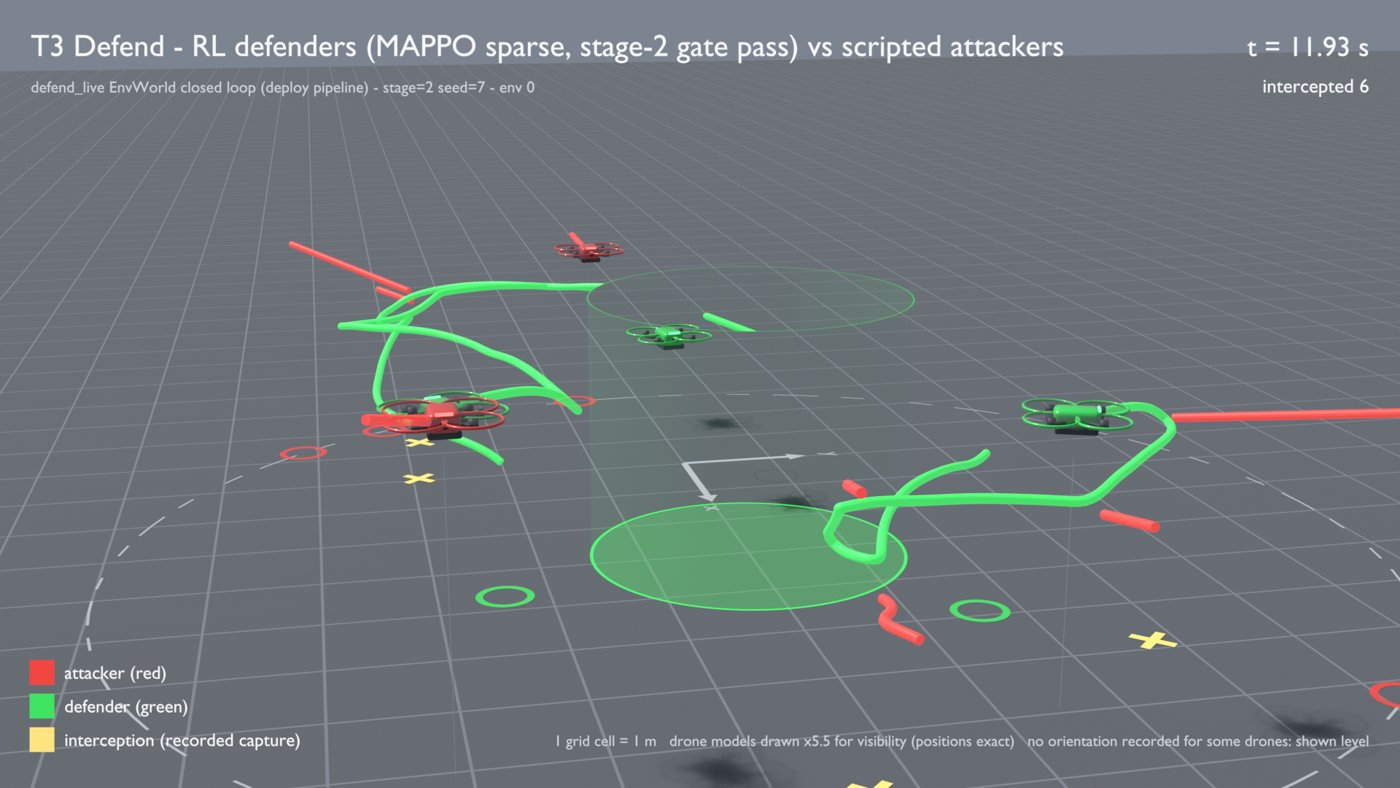
\includegraphics[width=\linewidth]{blender_defend.jpg}\caption{Defend S2}\end{subfigure}
\caption{Blender renders of recorded policy rollouts (\texttt{videos/blender/}). The trajectories come from the evaluation runs
and are validated against the recordings (\texttt{results/*\_validate.json}).}\label{fig:renders}
\end{figure}

\section{Deployment and safety}
\texttt{deploy/install.sh} copies our plug-ins into the organizers' checkout and registers \texttt{defend\_rl} and
\texttt{defend\_lead} in \texttt{swarm\_policies.py}. The run command is
\texttt{python3 swarm\_policies.py -{}-run defend\_rl:1,2,3 -{}-fly -{}-duration 120}.
These safety behaviours are always on:
\begin{itemize}
\item a geofence;
\item teammate separation;
\item hover when a pose is stale ($>1$\,s) or missing;
\item a per-axis speed clamp;
\item a dedicated altitude controller (target 1.8\,m, climb cap 60 rc units);
\item Ctrl+C lands all drones.
\end{itemize}
A hand-carry \texttt{frame\_check} policy verifies the AprilTag-to-sim frame conversion
(y-up/z-out, 1.22\,m origin) before any flight.

\section{Limitations and next steps}
\begin{itemize}
\item Stage-3+ attackers (faster, more numerous, evasive) are not yet beaten by RL in the deploy harness. The adaptive
curriculum is the planned route. Stage 7 policies (Aryan) reach a 90.8\% stop rate on a clean feed but collapse
on a delayed, noisy feed.
\item No real-flight gate has been completed yet. The venue map must be recalibrated on the day.
\item The 1v1 render clip uses the 3v2 configuration (a hard-coded attacker count). We will re-render it.
\end{itemize}

\section*{Reproduce}
\small
\begin{verbatim}
# deploy-path parity check (numpy only, ~2 s): expect ~8.1 downed/ep, 0% breach at stage 2
python drone_deployment_infra/defend_live.py --dry-run --feed stage:2 --episodes 16 --quiet \
    --policy rl --weights submission/policies/defend_rl_sparse_s2/policy.npz
# figures
python3 submission/plots/make_plots.py
# report
cd submission/report && latexmk -pdf report.tex
\end{verbatim}
\end{document}
